\documentclass{standalone}
\usepackage{tikz}

\begin{document}
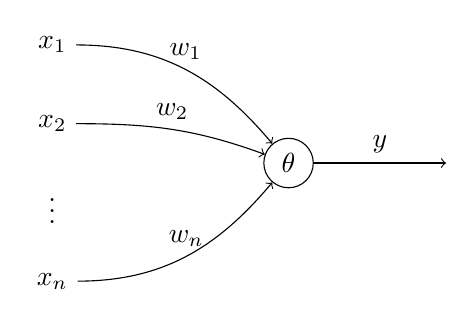
\begin{tikzpicture}
    \node[circle, draw] (f) at (0, 0) {$\theta$};
    \node (x1) at (-3, 1.5) {$x_1$};
    \node (x2) at (-3, .5) {$x_2$};
    \node (d1) at (-3, -.5) {\vdots};
    \node (xn) at (-3, -1.5) {$x_n$};

    \draw[->](x1)to[out=0,in=130]node[midway, above]{$w_1$}(f);
    \draw[->](x2)to[out=0,in=160]node[midway, above]{$w_2$}(f);
    \draw[->](xn)to[out=0,in=230]node[midway, above]{$w_n$}(f);
    \draw[->](f)--node[midway, above]{$y$}(2,0);
\end{tikzpicture}
\end{document}